% Document setup
\documentclass[a4paper, 11pt]{article}

% Packages
\usepackage{geometry}
\usepackage{amsmath}
\usepackage{subcaption}
\usepackage{graphicx}
\usepackage[table,xcdraw]{xcolor}
\usepackage[some]{background}
\usepackage{lipsum}
\usepackage[utf8]{inputenc}

% Break URLs in text and references
\usepackage{url}
\def\UrlBreaks{\do\/\do-} % Break on these characters
\usepackage{breakurl}
\usepackage[hidelinks, breaklinks]{hyperref}

\usepackage{float}
\usepackage{color}
\usepackage{booktabs}
\usepackage{longtable,lscape}

% Header setup
\usepackage{fancyhdr}
\usepackage[font=small,skip=10pt]{caption}
\usepackage{courier}

% Add unnumbered sections to toc
\usepackage[titletoc,toc,title]{appendix}

% Set up code listings
\usepackage{listings}
\lstset{ %
language=sh,                    % choose the language of the code
basicstyle=\footnotesize\ttfamily,breaklines=true,
numbers=left,                   % where to put the line-numbers
numberstyle=\footnotesize\ttfamily, % the size of the fonts that are used for the line-numbers
stepnumber=1,                   % the step between two line-numbers. If it is 1 each line will be numbered
numbersep=5pt,                  % how far the line-numbers are from the code
backgroundcolor=\color{light-gray},  % choose the background color. You must add \usepackage{color}
showspaces=false,               % show spaces adding particular underscores
showstringspaces=false,         % underline spaces within strings
showtabs=false,                 % show tabs within strings adding particular underscores
tabsize=2,                      % sets default tabsize to 2 spaces
captionpos=b,                   % sets the caption-position to bottom
breaklines=true,                % sets automatic line breaking
breakatwhitespace=false,        % sets if automatic breaks should only happen at whitespace
escapeinside={\%*}{*)}          % if you want to add a comment within your code
}
\definecolor{light-gray}{gray}{0.95}


\usepackage{fancyhdr}
\fancypagestyle{acknowledgements}
{
\fancyhf{}
\renewcommand{\headrulewidth}{1pt}%
\fancyhead[R]{\textsc{Acknowledgements}} % 1. sectionname
\fancyfoot[C]{\thepage}
}

\pagestyle{fancy}
\renewcommand{\sectionmark}[1]{\markboth{#1}{}} % set the \leftmark

\fancyhf{}
\fancyhead[R]{\textsc{\leftmark}} % 1. sectionname
\fancyfoot[C]{\thepage}
\fancypagestyle{plain}{%
  \fancyhf{}%
  \renewcommand{\headrulewidth}{0pt}%

}

\makeatletter
\def\printauthor{%
    {\large \@author}}
\makeatother

\author{%
	\vspace{.30cm}
    \textbf{Bram ter Borch} \\
    \texttt{\footnotesize bram.terborch@os3.nl}\vspace{35pt}
    \textbf{Siem Hermans} \\
    \texttt{\footnotesize siem.hermans@os3.nl}
    }

\begin{document}
\begin{titlepage}
\newgeometry{bottom=0.5cm}
\begin{center}
  \textbf{\huge Automated migration of configuration management systems \\}
  \vspace{.3cm}
  \Large \textit{A large-scale corporate fusion scenario}
  \\
  \vspace{.5cm}
  
\includegraphics[scale=1.2]{img/UvA-logo-english.jpg}
  \\
  \vspace{.5cm}
  \normalsize \textbf{LIA Research Project}
  \\
  \normalsize System and Network Engineering
  \\
  \vspace{.3cm}
  \normalsize {March 25, 2016}
  \vspace{.2cm}
\end{center}

\begin{figure}[!hb]
  \begin{center}
  	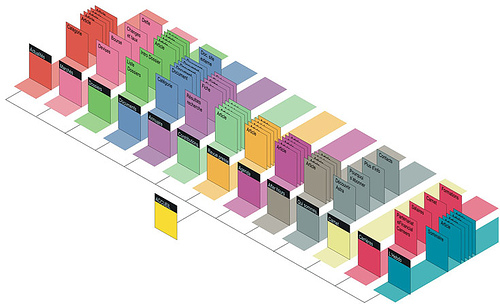
\includegraphics[scale=0.55]{img/cover.jpg}
  \end{center}
\end{figure}

\noindent
\begin{minipage}{0.28\linewidth}
    \begin{flushright}
        \printauthor
    \end{flushright}
\end{minipage} \hspace{8pt}
%
\begin{minipage}{0.02\linewidth}
	\vspace{1cm}
    \rule{1pt}{171pt}
\end{minipage} \hspace{-26pt}
%
\begin{minipage}{0.80\linewidth}
\vspace{5pt}
    \begin{abstract}
    \footnotesize
\noindent
Lorem ipsum dolor sit amet, consectetur adipiscing elit. Nullam sodales mauris eget mi porttitor tristique. Aliquam pharetra finibus mollis. Etiam dictum tempor nulla cursus vestibulum. Aliquam turpis quam, tincidunt eget lacus ac, suscipit laoreet sapien. Proin sed volutpat eros, et dignissim mi. Donec diam ipsum, pretium non vestibulum eget, porttitor nec risus. Quisque libero orci, convallis et neque et, interdum malesuada risus. Ut interdum efficitur gravida. Ut nec elementum quam. Nullam at finibus odio. Mauris condimentum maximus malesuada. Maecenas lobortis risus at sapien egestas cursus. Nunc a nibh bibendum, porttitor orci et, scelerisque erat. Phasellus dapibus finibus erat vitae rhoncus. Praesent lobortis enim id interdum commodo. Fusce vitae arcu id dolor mollis viverra at nec diam. Phasellus sodales magna non elementum malesuada. Donec ut lacinia mauris. Aliquam eu congue urna. Vestibulum lobortis varius feugiat.
    \end{abstract}
\end{minipage}
\begin{center}
  \vspace{.8cm}
%  \normalsize \textbf{Supervisor:}
%  \\
%  \normalsize Dr. Arno Bakker
%  \\

\end{center}

\end{titlepage}
\restoregeometry

%Table of Contents
\tableofcontents

\newpage

%Introduction
\section{Introduction}\label{sec:introduction}
Maintaining a consistent configuration across a large series of frequently changing systems can be a daunting task without the use of any configuration management tools. These tools  allow companies to automate deployments in a consistent manner and identify changes in hardware and software configuration or general infrastructure in a centralized manner. Most commonly, established tools such as Puppet\cite{whatispuppet}, Chef \cite{whatischef} and Ansible\cite{whatisansible} are used for this purpose. However, problems occur when two companies using different mechanisms to manage their systems need to merge. In the end, only one solution has to be selected, which requires a migration trajectory of some sort. An all or nothing approach is hard to perform as it has all the disadvantages which apply to any big bang migration. Therefore, we are interested in what needs to be done to make a gradual migration possible. We are mainly interested in whether it is possible to send commands with one configuration management tool to another, and as such transfer the management role between management systems in a gradual fashion. During the course of this project we will select two of the most popular systems and perform a transition in a small scale lab environment.
  


%Related  Work
\section{Related work}\label{sec:relatedwork}
Configuration management tools are a frequently researched topic by Enterprises, as their presence in an IT landscape  may lead to improvements in overall workflow. As these tools are mainly aimed at corporate infrastructures, the available literature commonly focuses on specific use cases from an Enterprise standpoint. Frequently these reports present use cases related to security aspects such as infrastructure hardening \cite{dotson2014security} or the repeatability of deployments \cite{ruiz2015reconstructable}. Additionally, as time progresses and new tools become available, product comparisons are drawn up. Hardion et al. \cite{Hardion2013} present a high level comparison of various configuration management tools on the market from the standpoint of a large research facility. Regarding the actual configuration of such tools, Collard et al. \cite{Collard2015} describe a method for verifying the configuration of Puppet. However, this paper exclusively focuses on environments with a single configuration management system. 

This research focuses on a migation trajectory in which a transition is made between Puppet and Ansible and vice versa, as corporate policy or functional requirements may dictate the final configuration management tool. Little official research related to this specific topic is currently available. Many parties only present a motivation for moving away from a given tool to a (usually) newer and more advanced tool. Dawson et al. \cite{dawson_hall_hecht_2014} presents such a motivation and argues that Ansible is superior to other tools with regards to deploying containers. Additionally, he identifies Puppet as one of the most influential configuration management tools of current time. Ansible as a tool is identified as a common migration target. 

On the topic of migation strategies, Zunker \cite{zunker_2014} goes into more depth in a blog post and presents a starting point for performing a gradual migration between Puppet and Ansible. He describes a conceptual method for piping output from Puppet to Ansible and talks about interpreting the output from each tool.

Moreover, as of late, new concepts for configuration management tools have been surfacing. \texttt{mgmt} by Shubin \cite{shubin2016} is a self proclaimed 'next generation' configuration management prototype.  Up until now, most configuration management tools have been employing a push or pull-based client-server model. \texttt{mgmt} uses a distributed architecture which allows for parallelization and a distributed topology. Due to the way \texttt{mgmt} is built, the tool may be suitable for a gradual migration trajectory.


\subsection{Background}\label{sec:background}
In this report we repeatedly talk about configuration management. Pressman \cite{pressman2005software} presents a definition for configuration management with regards to software engineering. He defines it as

``the task of tracking and controlling changes in the software, part of the larger cross-discipline field of configuration management.''

However, we expand this acronym to 


%Background Information
\section{Background}\label{sec:background}
As the line between system management and system orchestration is becoming thinner, configuration management tools are likely to be used for some orchestration purposes \cite{papazoglou2003service}. Additionally, all configuration management systems (CMS) are using either a push or a pull system to inform clients in case of updates. Lastly, \texttt{mgmt} is a new system which challenges the architectural model of established configuration management tools. This section presents a brief comparison of the selected configuration management tools and the distributed \texttt{mgmt}.

%added a citation about orchestration and SOA. Don't know if it is really related. But in a far distance it empowers the first line of this section.

\begin{lstlisting}[caption={Shellshock security patching with Ansible playbook},label=lst:shellshock]
- hosts: all
  gather_facts: yes
  remote_user: administrator
  sudo: yes
  tasks:
    - name: Update Shellshock (Debian)
      apt: name=bash
           state=latest
           update_cache=yes
      when: ansible_os_family == "Debian"
 
    - name: Update Shellshock (RedHat)
      yum: name=bash
           state=latest
           update_cache=yes
      when: ansible_os_family == "RedHat"
\end{lstlisting}

\subsection{Migration strategies}\label{subsec:migrationstrategies}
Migrating between systems can be done in different strategies and using different tooling, when using Configuration management system (CMS) A on all of the servers. New servers can be managed by CMS B. This will result in a slow migration between the management systems. The lifetime of a server dictates the time it will take to migrate, nowadays only the low level systems like NTP, DNS and authentication server should be bare metal servers. All other services depending on these could be virtual. The lifetime of these virtual servers is often less than the lifetime of bare metal machines because the virtual machines are created to support a specific service and are terminated directly when the service is no longer needed. Some special cases are excluded from this example, for instance a DHCP servers. When using virtual machines the migration process can be finished fast. In a cluster of 10 webservers managed by CMS A offering the same website, a new webserver could be created managed by CMS B. When tested and approved it can be added to the cluster. An old server should be removed from the cluster and decommissioned. In Large scale environments this will be an extensive job. Try doing this in a farm of a hundred web front-end servers.

\begin{quote}
According to Jaap van Ginkel on thursday 10-3-2016 during a lecture on Large Installation Administration, "More system administrators scale out services by using virtual machines"
\end{quote}

To keep server management easy and effective. One configuration management system should be used and the migration should not stretch multiple years. A Big bang scenario is a proper alternative. Migrating all the webservers from CMS A to CMS B by a set of automated steps without installing new servers. Therefore not using extra resources and migrating without downtime. This big bang scenario \cite{bigbang} is explained in this report as the focus of this report lays on Large Installation Administration.


\subsection{Orchestration and configuration management}\label{subsec:orchestration}
In this report we repeatedly discuss configuration management. As this term carries a somewhat ambiguous definition, we settle on the definition as presented by Pieter Lexis during a guest lecture at the University of Amsterdam. He defines configuration management as "the techniques and policies to track hardware, infrastructure and software, and the configuration thereof". During the course of this report we will use this definition exclusively.


\subsection{Differences between Push and Pull based management systems}\label{subsec:pushpull}
Puppet and Chef are pull based CMS's. A clients needs to be installed on the managed machine. This clients checks in at the server every x minutes. For puppet the default x time is 30 minutes. So every 30 minutes the configuration as it should be according to puppet is compared to the current configuration of the server. The puppet configuration can make sure a specific version of apache is installed or if a website contains a certain line of text. When the configuration differs from the configuration set in the Puppet configuration it will be changed immediately. Where Ansible and Salt use the push technique to send commands to a managed machine. Ansible uses playbook which hold the command set for specific server and it contains the destinations for the command set. The management server starts communication over SSH to the management machines and delivers and runs a python script on the client. So Python is a prerequisite for Ansible. The Python script is removed right after it is executed. This way of configuring servers is on demand. But as Puppet it is able to check for specific software versions or check file content and change it if needed. When a configuration differs from the configuration in the playbook. The client will be changed when the playbook is run by an administrator. So when a playbook is not run, the configuration could differ from the intended configuration for a long time. 

When a CMS only needs SSH to remote configure a machine, the scale of systems it could manage is a lot bigger than a client based system. If the system to manage has a closed operating system it cant be managed by a pull based CMS. All large networking brands make sure there operating systems (OS) are able to keep running for years without interruption. To make sure the system stays up the OS is closed down making sure no third party applications are able to disrupt the system. Push based systems only rely on a SSH connection. Ansible is capable of executing the python script on the server, therefore the requirement of python on the managed server is no longer there. This makes it possible to manage closed source network operating systems like Juniper or Cisco devices run. 

A router or switch could be set up with the necessary basics to make sure it can be placed at the designated location and is accessible over the network by SSH. Ansible can be set up to do the rest of the configuration. Running a playbook that will generate a base configuration for all the machines within the same class and check the running configuration to see if it matches. If it doesn't match. Ansible will change it. Next to configuration changes, depending on the brand of equipment, Ansible is capable of performing a code upgrade on network devices. Some of the new devices offer nonstop service upgrades \cite{NSSU}\cite{ISSU}, what actually means upgrading the system during office hours without any downtime (when everything is configured in a proper way and all requirements are matched). When the installed base of a specific brand and type is big enough automation of configuration or code changes have as much advantages on network devices as it has on server configuration.  

\subsection{Distributed configuration management}\label{subsec:distributedmgmt}
As previously alluded to, a relatively new configuration management tool on the horizon is \texttt{mgmt}. \texttt{Mgmt} is currently classified as a 'prototype next generation configuration management tool' and is developed by Shubin \cite{shubin2016}. The tool focuses on \textit{parallelization}, \textit{event driven changes} and most notably, a \textit{distributed architecture} \footnote{The source code for \texttt{mgmt} is available on GitHub: \url{https://github.com/purpleidea/mgmt/}}. 

\subsubsection{Distribution}
The main point of innovation in \texttt{mgmt} is the distributed topology of the system. As discussed in section \ref{subsec:pushpull}, traditional tools like Ansible and Puppet generally run in a client-server, push or pull manner. Naturally, as all code is placed in a central location, scalability and performance issues occur, especially when the amount of clients increases. Additionally, Shubin argues that using a client-server model reduces the configuration management tool to a single failure domain. Clustering of the master server could alleviate this problem, however, this would take away from the simplicity of a centralized system. Ansible on the other hand uses an orchestration model in which a push model is used. One of the most overlooked features in Puppet is the puppet executable. This allows you to both compile and apply catalogs locally, removing the complexity of running in client/server mode. However, as Shubin notes, this is a glorified method of running local scripts. Some users have opted not to use the Puppet master at all for scaling reasons. Although we feel that we have addressed most of these scaling issues with performance improvements in .25.x, the PuppetMaster will always be the bottleneck in client/server mode. For this deployment practice, users compile catalogs and apply configuration changes locally with the puppet executable. Code on all of the hosts is then kept in sync with a central repository using something like rsync. This will always be the best way to scale Puppet deployments, but it suffers from a loss in security as well as ease of management. This introduces new questions. With no puppetmasters, you have to allow *every* server to connect to your database instance. Another option would be to use a tiered Puppet Master system in which areas are defined. The top tier master would maintain other Puppet masters which in turn configure a set of clients. Similarly, Ansible can run in a local mode by specifiying the target to be the local machine. 

\subsubsection{Parallelization}
However, providing the option for parallel execution introduces room for errors as well. In a simple example, running two package installations with \texttt{apt} in parallel would fail due to a global lock on \texttt{dpkg}. Similarly, dependencies between applications and libraries would have to be resolved in a sequential manner. \texttt{Mgmt} deals with this scenario by batching (or grouping) all blocking operations and putting them in a sequential order. All operations which can be parallelized are placed in disjoint graphs as opposed to a directed acyclic graph. Parallelization does allow a system to reach its end state more rapidly. Long running processes which limited the deployment speed in a sequential process can now be converge quicker. In the setup for our experiment, the modules have direct dependencies. However, in a real world scenario it isn't uncommon for a company to have multiple disconnected modules without inter-dependencies run simultaneously. Tradeoff between safety and speed. 

%add images for parallel operations

\subsubsection{Event based model}
All the discussed configuration management systems have a notion of idempotence. In practice this means that the tools check the state of a certain element and compare it to a desired end state. If the state at time of checking has diverged from the desired state, the configuration will be altered by either a pull (Puppet) or push (Ansible) operation. In the context of Puppet this check operation is executed every 30 minutes by default. Ansible's push operation has to be manually scheduled with a \texttt{cronjob}. This mode of operation allows a configuration to diverge during the timeframe in which no check operation is performed. Naturally, a more preferable method would be to define an end state 

\subsubsection{Migration possibilities}
Another advantage which \texttt{mgmt} poses is that a migration between a tool like Puppet the tools could potentially be fairly easy. Converting Puppet modules to \texttt{mgmt} graphs is a straight forward process as displayed by ffrank \cite{}. However, due to the fact that \texttt{mgmt} still uses an experimental DSL, conversions at this point are mood. This is also exhibited by Frank \cite{}. 


%Method
start writing here


%Results
\section{Results}\label{sec:results}
In this section the outcomes of the applied migration strategy as designed in section \ref{sec:methodology} are discussed. Subsequently, results are presented for (re)convergence and parallel execution experiments in \texttt{mgmt}.

\subsection{Migration results}
The migration strategy as described in section \ref{sec:methodology} forms a large part of the results for this report. During the project the migration has been performed successfully in an automated fashion by creating a series of Ansible playbooks and Puppet modules. All created resources to make this migration possible have been made available in the appendices at the end of this report. Below are some migration specific results and key points which occured whilst performing the migration. 
\\\\
\noindent
\textbf{State definition mismatches}\\
In order to perform the migration of a node from Puppet to Ansible, the Puppet module defining the state of the Apache server has been converted to an Ansible playbook. The full Puppet module can be found in Appendix \ref{app:puppetmodule} and the Ansible playbook in Appendix \ref{app:ansibleplaybook}. A major factor of migrating a node between systems is the fact that all Puppet modules to be migrated need to be reproduced within Ansible playbooks (or vice versa). Special care has to be taken when reproducing these state definitions in either language as minor differences may cause downtime. In the state definitions used for the migration a mismatch occured in the installed Apache modules.
\\
\begin{lstlisting}[caption={Module mismatch in state definitions},label=puppetmod]
# Puppet module
class { 'apache':
     mpm_module => 'event',
}

# Ansible playbook
 - name: enabled mod_rewrite
        apache2_module: name=rewrite state=present
\end{lstlisting}

\noindent
The Puppet module as shown in listing \ref{puppetmod} contained a module which was not present in the Ansible playbook and the other way around. This caused a reinstallation of the \texttt{apache2} package when Ansible applied its playbook on the clients. Therefore, adding complexity may cause recompilation of the target service and cause unexpected downtime when the conversion process of modules to playbooks is not fully correct.
\\\\
\noindent
\textbf{Action handlers}\\
Additionally we examined irregular behavior between Ansible and Puppet due to the way commands are handled by each system. Puppet for example uses a semi-random execution model by design when applying a Puppet module, meaning that actions defined in a Puppet module may not be applied in a sequential order. This may cause problems when installing services and defining resources. For example, the Puppet module displayed in Appendix \ref{app:puppetmodule} installs the \texttt{apache2} package and defines content for the index.php and style.css files to be hosted by the webserver. Due to its order of execution, Puppet could potentially attempt to create the files (in non-existent directories) prior to installing Apache. Moreoever, Puppet -as opposed to Ansible- does \textit{not} stop applying a module when errors occur. This would mean that reaching the desired end state would require a second Puppet run, which by default is set to 30 minutes. As such a broken service is delivered for half an hour if a Puppet module definition is not sufficiently specific. 
\\
\begin{lstlisting}[caption={Code order regulation in Puppet},label=seqorder]
     file { '/tmp/uninstall.sh': 
        ensure => present,
        before => Exec['run_uninstaller'] 
     }
\end{lstlisting}

\noindent
Naturally, a relatively simple fix would be to define explicit relations between class definitions in the Puppet modules and resources. An example for this method is shown in listing \ref{seqorder} which is an excerpt from Appendix \ref{app:puppetmodule}. By using the \texttt{before} statement, the availability of the Puppet uninstaller is ensured prior to running the \texttt{run\_uninstaller} class. Still, when modules become more complex this would require a lot of extra code to be added, especially when modules are implemented in a hierachical structure. As opposed to Puppet, Ansible executes commands in the order as they are written in the playbook. In case of a failure the entire script is exited. When running the script again, it will start from the point where it failed last time. This makes an Ansible playbook easier to troubleshoot. Judging solely on these factors, Ansible fixes a series of issues present in Puppet, and as such is relatively easier to maintain in a large scale environment.
\\\\
\noindent
\textbf{Configuration mismatch window}\\
A push system like Ansible will connect to all of the clients targeted by a playbook to see if the configuration matches the required configuration as defined in the playbook. This make the architecture very easy to use, it has a low overhead and the only client side system requirement is to run an SSH server. However, this architecture also knows a downside. Ansible by default does not have a periodic push operation. When an environment has a large amount of playbooks and a specific playbook is not run periodically on certain machines, configuration changes can be made on local client system. Therefore not matching the rest of the servers with the same run. The difference will only be corrected when the appropriate playbook is run from the Ansible server, and only when the clients are placed in the correct groups. As for a pull based system the client checks in every 30 minutes (default for Puppet) and checks its configuration to the required configuration set by the master system. Still, proper placement of clients in groups is still required, as it should be, but the periodic check-in makes keeping a consistent environment easier. When changes are made to the system these changes will be corrected automatically. So unregistered changes will be overwritten as the configuration job regulates them. Important to note however is that when changes are made to parts which are not being regulated by the configuration management system, these changes will stay unnoticed and unchanged.
\\\\
\noindent
\textbf{Execution rights \& user interaction}\\
The described methodology requires that during a migration between two CMS's, both systems can talk to each other with the appropriate rights. Systems need to be removed from and added to specific configuration files. Therefore accounts that have the correct privileges need to be present at both environments. In a real world scenario this would generally be solved by having a central user database with rights management features. This could be a Lightweight Directory Access Protocol Database (LDAP) for example. 

Because this report aims to perform an automatic in-place migration, user interaction during the migration phase is not allowed. However, when new hosts are added to the management machines, some user action is often required for the acceptance of certificates for security reasons. For Puppet the way to allow all certificates is explained in section \ref{sec:methodology}. In summary, manual steps can be prevented by automatically accepting certificates from certain domains by utilising the \texttt{autosign.conf} file in Puppet. Ansible on the other hand uses certificates to login to the clients. So when the private key is protected by a password every playbook requires the password to be entered. As such, prior to migrating a certificate should be set up which omits the need for a password. Certificates are one of the most commonly used methods used by management solutions to connect to their clients. 

The proposed method in this report can be ran during production hours as the services on nodes being migrated will not be interrupted, assuming state definitions are correct. Naturally the state definitions need to be properly tested prior to performing any migration. By utilising the proposed method, the CMS a company is migrating away from will tell its clients to start communicating with a different CMS. The described method is also able to migrate a large number of machines at once by defining groups in either CMS, instead of migrating on a server by server basis which doesn't scale in large environments.

\subsection{\texttt{Mgmt} convergence speed}
Following the methodology as discussed in section \ref{sec:methodology} this section presents results on file convergence and package convergence. 
\\\\
\noindent
\textbf{File convergence}\\
Defining the desired state of individual (configuration) files in computer systems is a fundamental goal of configuration management systems. Listing \ref{fileconv} presents the run of a single node graph in \texttt{mgmt} which defines a generic file, '\texttt{file1}' and continuously monitors its state. The lower portion of the listing indicates that requesting the contents of the file, subsequently removing it and then requesting the contents again gives the same results for both \texttt{cat} commands. This is due to the fact that removing the file triggers an \texttt{inotify} event which makes \texttt{mgmt} re-check the file state with the CheckApply routine. The initial string value "Convergence test" is restored before the second \texttt{cat} command has a chance to run. In the code listing this happens at 15:26:05. This test indicates that file state convergence with \texttt{mgmt} in a limited size environment can be reached within a second.
\\
\begin{lstlisting}[caption={Rapid file convergence in \texttt{mgmt}},label=fileconv]
siem@development:~/mgmt$ ./run.sh run --file fileconv.yaml --graphviz=fileconv.dot
make: Nothing to be done for `build'.
[sudo] password for siem: 
15:25:26 main.go:65: This is: mgmt, version: 0.0.2-46-g7f3ef5b-dirty
15:25:26 main.go:66: Main: Start: 1458915926139787378
15:25:26 main.go:196: Main: Running...
15:25:26 main.go:106: Etcd: Starting...
15:25:26 configwatch.go:54: Watching: fileconv.yaml
15:25:26 etcd.go:132: Etcd: Watching...
15:25:26 config.go:248: Compile: Adding AutoEdges...
15:25:26 main.go:149: Graph: Vertices(1), Edges(0)
15:25:26 main.go:154: Graphviz: Successfully generated graph!
15:25:26 main.go:163: State: graphNil -> graphStarting
15:25:26 file.go:325: File[file1]: CheckApply(true)
15:25:26 main.go:165: State: graphStarting -> graphStarted
15:26:05 file.go:325: File[file1]: CheckApply(true)  # Check file state
15:26:05 file.go:363: File[file1]: Apply             # Apply desired state 
15:26:13 main.go:51: Interrupted by ^C
15:26:13 pgraph.go:559: File[file1]: Exited
15:26:13 main.go:209: Goodbye!

siem@development:~$ cat file1 && sudo rm file1 && cat file1 
Convergence test                                     # Timestamp: 15:26:05
Convergence test                                     # Timestamp: 15:26:05
siem@development:~$ 
\end{lstlisting}
\noindent
It should be noted however that the \texttt{etcd} master in this scenario is located on the node hosting the file. In a real world scenario with a hierarchical implementation of the \texttt{etcd} store, communication would be required between the node and the \texttt{etcd} instance to request the current state of the key-value pair (assuming the node hosting the file is not an \texttt{etcd} leader node). Still, rapid convergence of (configuration) files in the range of several seconds is a leap forward from periodic checking of the desired state.
\\\\
\noindent
\textbf{Package convergence}\\
After testing file convergence in \texttt{mgmt} parallel execution and package convergence is examined. Listing \ref{packconv} shows the creation of graph as based on figure \ref{fig:parallelexec} with its seven vertices and six edges based on the \texttt{pkg1.yaml} resource graph file. The full configuration file for this specific test scenario is available in appendix \ref{app:mgmtgraph}.
\\
\begin{lstlisting}[caption={Graph initiation for package convergence},label=packconv]
siem@development:~/mgmt$ ./run.sh run --file pkg1.yaml --graphviz=output.dot
[...] # Output omitted
14:12:25 configwatch.go:54: Watching: pkg1.yaml
14:12:25 etcd.go:132: Etcd: Watching...
14:12:27 config.go:248: Compile: Adding AutoEdges...
14:12:27 main.go:149: Graph: Vertices(7), Edges(6)
14:12:27 main.go:152: Graphviz: output.dot
14:12:27 main.go:163: State: graphNil -> graphStarting
14:12:27 main.go:165: State: graphStarting -> graphStarted
[...] # Output omitted
14:12:27 pkg.go:208: Pkg[apache2]: CheckApply(true)
14:12:29 pkg.go:259: Pkg[apache2]: Apply
14:12:29 pkg.go:266: Pkg[apache2]: Set: installed...      # Initiate install
14:12:47 packagekit.go:417: PackageKit: Timeout: InstallPackages: Waiting for 'Destroy'
14:12:47 pkg.go:284: Pkg[apache2]: Set: installed success!  # Finish install
\end{lstlisting}
\noindent
At this point the graph is initiated and the \texttt{apache2} package has been installed. This is also visualized in the lower section of listing \ref{packconv}. Subsequently, in listing \ref{remconv}, the \texttt{apache2} package is removed which triggers a PackageKit event (which is linked to \texttt{dbus}), eventually causing \texttt{mgmt} to reinstall the package. 
\\
\begin{lstlisting}[caption={PackageKit convergence in \texttt{mgmt}},label=remconv]
14:13:33 pkg.go:208: Pkg[apache2]: CheckApply(true)
14:13:35 pkg.go:259: Pkg[apache2]: Apply
14:13:35 pkg.go:266: Pkg[apache2]: Set: installed...

siem@development:~$ service apache2 status     # Service status (initial run)
 * apache2 is running
siem@development:~$ sudo apt remove --purge -y apache2  # Timestamp: 14:12:50
siem@development:~$ service apache2 status
apache2: unrecognized service
siem@development:~$ service apache2 status              # Timestamp: 14:13:35
 * apache2 is running
\end{lstlisting}

\noindent
Judging by the timestamps it takes circa 45 seconds from the point of removing the package to have \texttt{apache2} operational again in its intended state. Naturally, the time it takes to reconverge is largely dependent on the type of package being installed and the amount of dependencies of the package. Within \texttt{mgmt}, in general, reaching the desired state for the installed packages on a system is significantly slower than file reconvergence. However, considering the fact that traditional push and pull based systems can't realistically poll within sub-minute timeframes, \texttt{mgmt} still outperforms traditional systems significantly.  



%Conclusion and discussion
\section{Conclusion}\label{sec:conclusion}
When corporate merges take place, the IT department is commonly one of the first departments that needs to merge. As IT environments are continuously growing in size and complexity these merges come with great challenges, especially when a core component like a configuration management system has to be merged. This paper looks into migrating nodes between configuration management systems for server management in case of a corporate merge scenario. A method for performing an in place migration between a pull- and a push-based configuration management system is presented. More specifically, the implications of migrating a node from being managed by Puppet to Ansible and vice versa are examined. During this process the prerequisites for performing an automated migration are identified. Additionally the current state of the relatively new and distributed configuration management system \texttt{mgmt} is assesed and the possibilities of migrating to this system in the future are discussed.

In order to perform a successful automated in-place migration  a migration model based on a friendly takeover is proposed. In this model the legacy system gradually removes itself prior to the new CMS taking over the nodes. During the project a virtual lab environment has been set up to verify whether the proposed model works in practice. Ansible playbooks and Puppet modules have been defined which can perform this migration in an automated fashion. The main advantages of utilizing the proposed method is that at no point in time the nodes to be migrated become unmanaged. Moreover, by performing a friendly takeover a clean migration whilst maintaining proper error reporting can be achieved. Technical constraints during the migration could easily be overcome which makes the model a good framework for this specific type of merge. 

With regards to \texttt{mgmt} our experiments show that this prototype CMS introduces significant advantages over traditional configuration management systems. However, due to its prototype status a full migration path at this point in time is not feasible. Scalability and stability experiments have to be performed prior to fully deploying the software in a large scale production environment. Still, developments are moving forward rapidly and the language used by \texttt{mgmt} is similar to Ansible. This means that in the near future a natural migration path from a push based system to a distributed system becomes feasible. We conclude on the notion that an in place migration on production machines is feasible without any perceivable effect for end users by leveraging the migration model as presented in this report. However, performing any kind of migration between configuration management systems is heavily dependent on the architectural model of the tool in place. Therefore, extrapolating the migration model as presented in this report to a generic model would be ill advised. 


\subsection{Future Work}\label{subsec:futurework}
Although this report does not primarily focus on migrating to \texttt{mgmt}, it is undeniably an impressive development. As this new configuration management system is still in an experimental phase, it does not have a definitive Domain Specific Language in place yet which means that migrating to a distributed CMS would be too risky for now. However, when the development of \texttt{mgmt} takes on a more permanent form, it would be interesting to see how a migration from a Client-Server CMS like Puppet or Ansible to \texttt{mgmt} would play out. Frank \cite{frank_2016} provides a starting point for transpiling Puppet modules to \texttt{mgmt} resource graphs by using a series of complex regular expressions. However, further investigation on streamlining this process is required.

Additionally, this research looked into only a small part of migrating a corporate IT infrastructure between Puppet and Ansible. We opted to migrate an Apache web server, as this product has extensive documentation and was readily available. The methodology posed was able to perform an in-place migration without any downtime. However, in order to do so the Puppet module had to be manually converted to an Ansible playbook and vice versa. To speed up migrations it would be beneficial to automate this conversion process. Work is currently being done by Nigmatullin and Van Dijk \cite{marat_2016} to automate the creation of these playbooks and modules from a static configuration, but it would be advisable to perform a consistency and stability analysis of this method prior to applying it in a production environment. 

Lastly, we primarily focused on managing generic virtual machine instances with Puppet and Ansible and did not take (Docker) containerization into consideration. Deploying Docker containers on a large scale is currently primarily being done via Dockerfiles, which contain a sequence of pre-defined commands in order to deploy a service with a given configuration. Scalability issues occur when the services to be deployed become overly complex and require a large set of commands. At that point they require relatively static and unmanageable Dockerfiles. Configuration management tools like the ones discussed in this report are currently working towards supporting fine-grained configuration management features for various types of container platforms. However, as such features become available the line between orchestration tools like Kubernetes \cite{kubernetes_2016} and configuration management systems becomes less obvious. It would be interesting to see how orchestration tools at this point in time relate to configuration management systems and whether a distinction would still be relevant in the near future.


%Future work
\section{Future work}\label{sec:futurework}
This report primarily focuses on managing generic virtual machine instances with Puppet and Ansible and does not take Docker containerization in consideration. Deploying Docker containers on a large scale is currently primarily being done via Dockerfiles, which contain a sequence of pre-defined commands in order to deploy a service with a given configuration. Problems occur when the services to be deployed become overly complex and require a large set of commands. At that point they require relatively static and unmanageable Dockerfiles. Configuration management tools like the ones discussed in this report are currently looking into supporting fine-grained configuration management features for various types of container platforms. However, as such features become available the line between 'true' orchestration tools like Kubernetes \cite{kubernetes_2016} become less obvious. It would be interesting to see how orchestration tools at this point in time relate to configuration management tools and whether a clear distinction can be made in the near future.

Although we don't focus on \texttt{mgmt} in detail in this report, it is undeniably an interesting development. As this new tool is still in an experimental phase, it does not have a definitive Domain Specific Language in place yet. This means that a migration strategy to a distributed model is currently out of scope. However, when the development of \texttt{mgmt} takes on a more solid form, it would be interesting to see how a migration from Puppet to \texttt{mgmt} would play out. James \cite{frank_2016} provides a starting point for transpiling Puppet modules to \texttt{mgmt} resource graphs by using a series of complex regular expressions. However, further investigation on this topic is required.


%Acknowledgements
\thispagestyle{acknowledgements}
\addcontentsline{toc}{section}{Acknowledgements}
\section*{Acknowledgements}\label{sec:acknowledgements}
We would like to thank our colleague Peter Boers for providing us with a quick and concise crash course on writing and modifying Puppet modules. Furthermore we would like to thank Auke Folkerts for providing us with information on the topic of configuration management systems in general and migration strategies specifically. Lastly we thank Pieter Lexis for his rapid response times regarding technical questions and for providing us information on \texttt{mgmt}.


\cleardoublepage
\begingroup

\addcontentsline{toc}{section}{References}

\begingroup
\raggedright
\bibliographystyle{unsrt}
\bibliography{report}
\endgroup

%Appendices
\begin{appendices}
  \renewcommand\thetable{\thesection\arabic{table}}
  \renewcommand\thefigure{\thesection\arabic{figure}}

  \section{Puppet Apache module} \label{app:puppetmodule}
  \begin{lstlisting}
   # This class definition depends on the puppetlabs/apache module
   class pe_apache_app {

   class { 'apache':
     mpm_module => 'prefork',
   }

   include apache::mod::php

   apache::vhost { 'pe_apache_app':
     port     => '80',
     docroot  => '/var/www/',
     priority => '10',
   }

   file { '/var/www/pe_apache_app/index.php':
     ensure  => file,
     content => "This server is managed by Puppet!",
     mode    => '0644',
   }
 }
  \end{lstlisting}
  \newpage

  \section{Puppet agent removal} \label{app:puppetagent}
  \begin{lstlisting}
  
  \end{lstlisting}
  
  \newpage  
  \section{Ansible migration playbook} \label{app:ansiblemigration}
  \begin{lstlisting}
  ---
  - hosts: slave02
    sudo: yes
    tasks:
     - lineinfile: dest=/etc/hosts line="172.16.175.131 puppet-master.puppet.local" state=present
     - name: Install puppet agent
       shell: curl -k https://puppet-master.puppet.local:8140/packages/current/install.bash | sudo bash
  \end{lstlisting}

  \newpage
  \section{Ansible apache playbook} \label{app:ansibleplaybook}
  \begin{lstlisting}
    ---
    - hosts: webservers
      sudo: yes
      tasks:
        - name: install apache2
          apt: name=apache2 update_cache=yes state=latest

        - name: enabled mod_rewrite
          apache2_module: name=rewrite state=present
          notify:
            - restart apache2

        - name: delete old apache index.html
          file: path=/var/www/html/index.html state=absent

        - name: create new awesome index.php
          file: path=/var/www/html/index.php state=file

        - lineinfile: dest=/var/www/html/index.php regexp='.' state=absent
        - lineinfile: dest=/var/www/html/index.php line="This machine is managed by Ansible!" state=present
          notify:
            - restart apache2

    handlers:
      - name: restart apache2
        service: name=apache2 state=restarted
  \end{lstlisting}

\end{appendices}




\end{document}
